\section{Natural Language Processing}\label{sec:nlp}
%**************************************************************

The field of \gls{nlp}, also known as computational linguistics, is a branch of Artificial Intelligence focused on the technology of processing language.
It encompasses a variety of topics, which involves the engineering of computational models and
processes to solve practical problems in understanding and generating human
languages. These solutions are used to build useful software.

The linguistics computational has two
branches---computational linguistics and theoretical linguistics. The computational
linguistics has been concerned with developing algorithms for handling a useful
range of natural language as input. While the theoretical linguistics has focused
primarily on one aspect of language performance, grammatical competence---how
people accept some sentences as correctly following grammatical rules and others as ungrammatical. They are concerned with language universals—principals of
grammar which apply to all natural languages \cite{Cole:1996}.

Computational linguistics is concerned with the study of natural language analysis
and language generation. Further, the language analysis is divided into two domains,
namely sentence analysis, and discourse and dialogue structure. Much more is known
about the processing of individual sentences than about the determination of discourse
structure. Any analysis of discourse structure requires a prerequisite as an analysis of
the meaning of individual sentences. However, it is a fact that for many applications,
thorough analysis of discourse is not mandatory, and the sentences can be understood
without that \cite{grishman_computational_1986}.

The sentence analysis is further divided into syntax analysis and semantic analysis.
The overall objective of sentence analysis is to determine what a sentence "means".
In practice, this involves translating the natural language input into a language with
simple semantics, for example, formal logic, or into a database command language.
In most systems, the first stage is syntax analysis. Figure \ref*{fig:nlp_components} shows the relations
among different components of NLP \cite{Chowdhary2020}.

\begin{figure}[H]
    \centering
    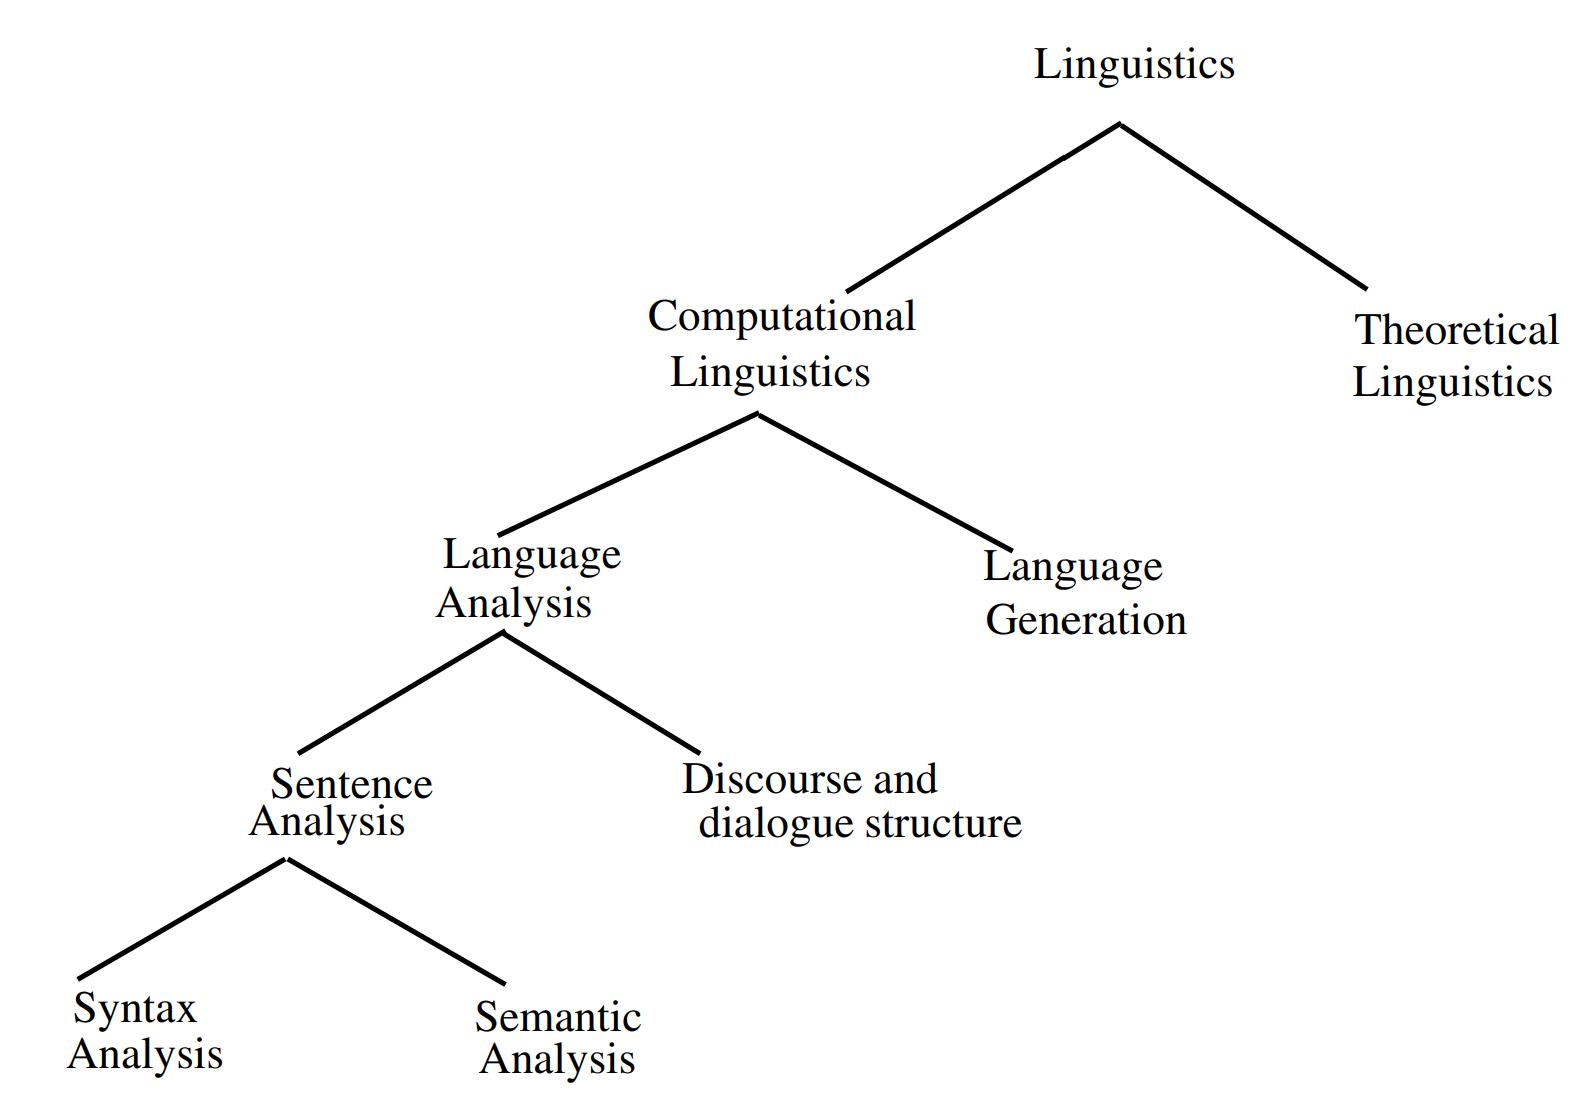
\includegraphics[width=\textwidth]{images/2_1_nlp_components.png}
    \caption{Components of NLP}\label{fig:nlp_components}
\end{figure}
    


Some of the common applications of NLP are: Classification of text into categories, Index and search large texts, Automatic translation, Information extraction,
Automatic summarization, Question answering, Knowledge acquisition, and Text
generations/dialogues.
Some of those tasks are discussed in sections \ref{subsec:text-classification}, \ref{subsec:sentiment-analysis}, \ref{subsec:nli}, \ref{subsec:seq2seq}.


%**************************************************************
\subsection{Text classification}\label{subsec:text-classification}

Classification lies at the heart of both human and machine intelligence. Deciding what letter, word, or image has been presented to our senses, recognizing faces or voices, sorting mail, assigning grades to homeworks; these are all examples of assigning a category to an input.
In this section we introduce text classification, the task of assigning a label or category to an entire text or document.

Given a text document, assign it a discrete label $y \in Y$, where $Y$ is the set of possible labels. 
Text classification has many applications, from spam filtering to the analysis of electronic health records, or the categorization of news articles.

Classification is essential for tasks below the level of the document as well.
An example of this is period disambiguation (deciding if a period is the end of a sentence or part of a word), or word tokenization (deciding if a character should be a word boundary). Even language modeling can be viewed as classification: each word can be thought of as a class, and so predicting the next word is classifying the context-so-far into a class for each next word. A part-of-speech tagger classifies each occurrence of a word in a sentence as, e.g., a noun or a verb.

The goal of classification is to take a single observation, extract some useful features, and thereby classify the observation into one of a set of discrete classes.

One method for classifying text is to use handwritten rules. There are many areas of language processing where handwritten rule-based classifiers constitute a state-ofthe-art system, or at least part of it. Rules can be fragile, however, as situations or data change over time, and for
some tasks humans aren't necessarily good at coming up with the rules. Most cases of classification in language processing are instead done via supervised machine learning, where an algorithm learn how to map from an observation to a correct output \cite{Jurafsky2009}.

Many kinds of machine learning algorithms are used to build classifiers.
Formerly, statistical and machine learning approaches, such as naïve Bayes, k-nearest neighbors, hidden Markov models, conditional random fields (CRFs), decision trees, random forests, and support vector machines, were widely used to design classifiers. 
However, during the past several years, there has been a wholesale transformation, and these approaches have been entirely replaced, or at least enhanced, by \gls{nn} models \cite{journals/corr/abs-1807-10854}. 

%**************************************************************
\subsection{Sentiment analysis}\label{subsec:sentiment-analysis}
A popular application of text classification is sentiment analysis, the extraction of sentiment, the positive or negative orientation that a writer expresses toward some object. A review of a movie, book, or product on the web expresses the author's sentiment toward the product, while an editorial or political text expresses sentiment toward a candidate or political action. Extracting consumer or public sentiment is thus relevant for fields from marketing to politics. 

The simplest version of sentiment analysis is a binary classification task, and
the words of the review provide excellent cues. Consider, for example, the following phrases extracted from positive and negative reviews of movies and restaurants. Words like great, richly, awesome, and pathetic, and awful and ridiculously are very informative cues:

\textit{+ ...zany characters and richly applied satire, and some great plot twists}

\textit{− It was pathetic. The worst part about it was the boxing scenes...}

\textit{+ ...awesome caramel sauce and sweet toasty almonds. I love this place!}

\textit{− ...awful pizza and ridiculously overpriced...} 

\cite{Jurafsky2009}
%**************************************************************

\subsection{Natural language inference}\label{subsec:nli}

%**************************************************************

\subsection[Seq2Seq]{Sequence-to-Sequence models}\label{subsec:seq2seq}

%**************************************************************

\subsection{Lexicon}\label{subsec:lexicon}

%**************************************************************

\subsection{Word Embeddings}\label{subsec:word-embeddings}

%**************************************************************

\subsection{Masked Language Models}\label{subsec:masked-language-models}

%**************************************************************